\chapter{{\sffamily SK} Combinators}
%\vspace{2cm}
\vspace{1cm}

In this chapter we shall examine another graph reduction technique based on
a \textit{fixed set of supercombinators}. The most important members of this set are
called \ml{S} and \ml{K}; hence the title of this chapter. The idea of having a fixed set of
supercombinators contrasts with the approach previously described, in which
the supercombinator definitions are generated from the program.

The method is appealing because it gives rise to an extremely simple
reduction machine which, in effect, only has to support built-in operators and
needs no template-instantiation mechanism. In addition it turns out that the
implementation is, in a certain sense, lazier than our best efforts so far, but as
we shall see, these benefits are won at a price.

(Note: in this chapter we shall use lower-case letters to stand for
expressions, to avoid confusion with the combinators, which are written in
upper case.)

\section{The {\sffamily SK} Compilation Scheme}

Our strategy is to transform the program into one containing only the built-in
operators and constants, together with the combinators \ml{S}, \ml{K} and \ml{I}. These
combinators are described by the reduction rules
\begin{letalign}
    S f g x &$\rightarrow$ f x (g x) \\
    K x y &$\rightarrow$ x \\
    I x &$\rightarrow$ x
\end{letalign}
The motivation for choosing this particular set should become clearer as we
proceed. \ml{S}, \ml{K} and \ml{I} are all supercombinators, since they satisfy the definition
given in Chapter~13, but for the purposes of this chapter, and for compatibility
with other published work, we will use the more general term `combinator'.

\subsection{Introducing \ml{S}, \ml{K} and \ml{I}}

Consider the lambda abstraction \ml{Fun}, where
\begin{letalign}
    \ml{Fun} &= \ml{(\tlb{x}$e_1$ $e_2$)}
\end{letalign}
where $e_1$ and $e_2$ are arbitrary expressions. Given the reduction rule for \ml{S}, an
equivalent expression is \ml{Fun'}, where
\begin{letalign}
    \ml{Fun'} &= \ml{S (\tlb{x}$e_1$) (\tlb{x}$e_2$)}
\end{letalign}
We can demonstrate that \ml{Fun} and \ml{Fun'} are equivalent by applying them to the
same argument:
\begin{mlcoded}
    \begin{tabular}{@{}l@{ }c@{ }l@{}}
        Fun arg & $=$ & $(\lambda x.\,e_1\; e_2)$ arg \\
        & $\rightarrow$ & ($e_1$[arg/x]) ($e_2$[arg/x]) \\[6pt]
        Fun' arg & $=$ & S $(\lambda x.\,e_1)$ $(\lambda x.\,e_2)$ arg \\
        & $\rightarrow$ & $((\lambda x.\,e_1)$ arg) $((\lambda x.\,e_2)$ arg) \\
        & $\rightarrow$ & ($e_1$[arg/x]) ($e_2$[arg/x])
    \end{tabular}
\end{mlcoded}
Hence \ml{Fun} $=$ \ml{Fun'} by extensional equality.

We call the transformation from \ml{Fun} to \ml{Fun'} the \ml{S}-\textit{transformation}, and
denote it using a `$\Rightarrow$'
arrow, in the following way:
\begin{letalign}
    \tlb{x}$e_1\; e_2$ &$\Rightarrow$ \ml{S} $(\lambda x.\,e_1)$ $(\lambda x.\,e_2)$
\end{letalign}
Notice the difference between the arrows `$\Rightarrow$'
and `$\rightarrow$'. Both denote the
transformation of one expression into an equivalent one, but the former
denotes a compile-time transformation and the latter denotes a run-time
reduction.

As an example of the use of the \ml{S}-transformation, consider the expression
\begin{letalign}
    \ml{h} &= \ml{\tlb{x}OR x TRUE}
\end{letalign}
Applying the \ml{S}-transformation twice, we get
\begin{mlcoded}
    \begin{tabular}{@{}l@{\;\;}c@{\;\;}l@{}}
        & & \tlb{x}OR x TRUE \\
        S & $\Rightarrow$ & S (\tlb{x}OR x) (\tlb{x}TRUE) \\
        S & $\Rightarrow$ & S (S (\tlb{x}OR) (\tlb{x}x)) (\tlb{x}TRUE)
    \end{tabular}
\end{mlcoded}
(We use an `\ml{S}' in the left margin to indicate that the \ml{S}-transformation rule is
being used.)

As we perform the \ml{S}-transformation, the \ml{\tl{}x} gets pushed down one level
each time, because so long as its body is an application we can apply the
\ml{S}-transformation again. Each time we apply the \ml{S}-transformation we produce
two new \ml{\tl{}x} abstractions, but with smaller bodies. In the end the body will be
an atomic object, and there are two cases to consider:


\begin{numbered}
    \item The expression is \ml{(\tlb{x}x)}. This is just the identity function, which we call \ml{I},
    with the definition
    \begin{letalign}
        \ml{I x} &$\rightarrow$ \ml{x}
    \end{letalign}
    The \ml{I}-transformation replaces \ml{(\tlb{x}x)} with \ml{I}, thus:
    \begin{letalign}
        \tlb{x}x &$\Rightarrow$ \ml{I}
    \end{letalign}
    There was an instance of this in the previous example, and applying the
    \ml{I}-transformation, we would get
    \begin{mlcoded}
        \begin{tabular}{@{}l@{\;\;}l@{\;\;}l@{}}
            & & S (S (\tlb{x}OR) (\tlb{x}x)) (\tlb{x}TRUE) \\
            I & $\Rightarrow$ & S (S (\tlb{x}OR) I) (\tlb{x}TRUE)
        \end{tabular}
    \end{mlcoded}

    \item The expression is \ml{(\tlb{x}c)}, where \ml{c} is a constant or a variable other than \ml{x}.
    This is a function which takes one argument, discards it, and returns \ml{c}, so
    we can replace it with \ml{(K c)}, where
    \begin{letalign}
        \ml{K c x} &$\rightarrow$ \ml{c}
    \end{letalign}
    The \ml{K}-transformation rule is therefore:
    \begin{letalign}
        \tlb{x}c &$\Rightarrow$ \ml{K c}
    \end{letalign}
    where \ml{c} is any constant, or a variable other than \ml{x}. As in the case of \ml{S}, the
    equivalence of \ml{(\tlb{x}c)} and \ml{(K c)} can be shown by extensional equality.

    \phantom{xx} There are two instances of this in our example, \ml{(\tlb{x}OR)} and \ml{(\tlb{x}TRUE)}.
    Replacing these with \ml{(K OR)} and \ml{(K TRUE)} we get
    \begin{mlcoded}
        \begin{tabular}{@{}l@{\;\;}l@{\;\;}l@{}}
            & & S (S (\tlb{x}OR) I) (\tlb{x}TRUE) \\
            K & $\Rightarrow$ & S (S (K OR) I) (K TRUE)
        \end{tabular}
    \end{mlcoded}
\end{numbered}

\noindent
To summarize, we have developed the \textit{transformation rules} and the \textit{reduction
    rules} for the combinators \ml{S}, \ml{K} and \ml{I} shown in Figure~16.1.

\boxedfigure{
    \noindent
    \begin{tabular}{@{}l@{\hspace{3cm}}l}
        S-reduction:       & \ml{S f g x} $\rightarrow$ \ml{f x (g x)} \\
        K-reduction:       & \ml{K c x} $\rightarrow$ \ml{c}         \\
        I-reduction:       & \ml{I x}  $\rightarrow$ \ml{x}         \\[6pt]
    \end{tabular}\\
    \begin{tabular}{@{}l@{\hspace{2.2cm}}l@{\quad}l@{\quad}l@{}}
        I-transformation:  & \tlb{x}x     & $\Rightarrow$ & \ml{I}         \\
        K-transformation:  & \tlb{x}c     & $\Rightarrow$ & \ml{K c} \qquad (\ml{c} $\neq$ \ml{x}) \\
        S-transformation:  & \tlb{x}$e_1\;e_2$ & $\Rightarrow$ & \ml{S} $(\lambda x.\,e_1)$ $(\lambda x.\,e_2)$
    \end{tabular}
}{The SKI rules}

We can use the reduction rules to evaluate the transformed program:
\begin{mlcoded}
    \begin{tabular}{@{}l@{\qquad }c@{\quad}l@{}}
        & & h x \\
        & $=$ & S (S (K OR) I) (K TRUE) x \\
        S & $\rightarrow$ & S (K OR) I x (K TRUE x) \\
        S & $\rightarrow$ & K OR x (I x) (K TRUE x) \\
        K & $\rightarrow$ & OR (I x) (K TRUE x) \\
        I & $\rightarrow$ & OR x (K TRUE x) \\
        K & $\rightarrow$ & OR x TRUE
    \end{tabular}
\end{mlcoded}
(We use an \ml{S}, \ml{K} or \ml{I} in the left margin as a reminder of which reduction rule is
being used.)

\subsection{Compilation and Implementation}

The \ml{S}, \ml{K} and \ml{I} transformations together constitute a complete compilation
algorithm (the \textit{\ml{SK} compilation algorithm}), which will transform \textit{any} lambda
expression into an expression involving only \ml{S}, \ml{K}, \ml{I} and constants!

Here, then, is the \ml{SK} compilation algorithm to compile an expression \ml{e}:

\plainbox{
    \noindent\ml{WHILE e contains a lambda abstraction DO}
    \vs
    \begin{compactenum}[\quad(1)]
        \item Choose any innermost lambda abstraction of \ml{e}.
        \item If its body is an application, apply the \ml{S}-transformation.
        \item Otherwise its body must be a variable or constant, so apply
        the \ml{K} or \ml{I} transformation as appropriate.
    \end{compactenum}
    \vs
    \noindent\ml{END}
}

\noindent
By transforming the innermost lambda abstractions first we ensure that the
body of the chosen lambda abstraction contains no lambdas. This, incidentally, means that we do not run into any \ml{\ta{}}-conversion problems, either during
compilation or evaluation of the combinator expression; a very desirable
property in view of the subtle problems encountered in Chapter~2.

As an example, let us compile the expression \ml{((\tlb{x}+ x x) 5)}.
\begin{mlcoded}
    \begin{tabular}{@{}c@{\qquad}l@{\quad}l@{}}
        & & (\tlb{x}$+$ x x) 5 \\
        S & $\Rightarrow$ & S (\tlb{x}$+$ x) (\tlb{x}x) 5 \\
        S & $\Rightarrow$ & S (S (\tlb{x}$+$) (\tlb{x}x)) (\tlb{x}x) 5 \\
        I & $\Rightarrow$ & S (S (\tlb{x}$+$) I) (\tlb{x}x) 5 \\
        I & $\Rightarrow$ & S (S (\tlb{x}$+$) I) I 5 \\
        K & $\Rightarrow$ & S (S (K $+$) I) I 5
    \end{tabular}
\end{mlcoded}
The successive lines show the state of the expression at successive iterations of
the algorithm's \ml{WHILE} loop. To reassure ourselves that the algorithm has
produced an equivalent expression, we can evaluate the result using the
reduction rules for the combinators:
\begin{letalign}
    & \ml{S (S (K +) I) I 5} \\
    $\rightarrow$ & \ml{S (K +) I 5 (I 5)} \\
    $\rightarrow$ & \ml{K + 5 (I 5) (I 5)} \\
    $\rightarrow$ & \ml{+ (I 5) (I 5)} \\
    $\rightarrow$ & \ml{+ 5 (I 5)} \\
    $\rightarrow$ & \ml{+ 5 5} \\
    $\rightarrow$ & \ml{10}
\end{letalign}

To summarize, we have developed a compilation algorithm which will
compile any expression into an expression involving only \ml{S}, \ml{K}, \ml{I} and constants
(including built-in functions). All the variables have disappeared! Recursion
may be dealt with using \ml{Y}, as previously explained in Chapter~6. \ml{Y} is then
treated as a built-in function by the combinator compilation algorithm.

\boxedfigure{
    \begin{tabular}{@{}l@{\qquad}l@{}}
        Name                            & Syntactic object \\[6pt]
        \ml{e}, \ml{e}$_1$, \ml{e}$_2$ & Expressions \\[6pt]
        \ml{f}, \ml{f}$_1$, \ml{f}$_2$ & Expressions with no inner \ml{\tl}s \\
        \ml{x}                          & A variable \\
        \ml{cv}                         & A constant (including function constants, such as \ml{+}, \ml{Y}, \\
        & etc.), or a variable \\
    \end{tabular}
    \vs

    \hdashsep
    \vs

    \phantom{XX} \metafnbb{C}{e} \quad {\bf C}ompiles \ml{e} to \ml{SK} combinators
    \vs

    \begin{letalign}
        \metafnbb{C}{e$_1$ e$_2$} &$=$ \metafnbb{C}{e$_1$} \metafnbb{C}{e$_2$} \\
        \metafnbb{C}{\tlb{x}e} &$=$ \metafn{A} \ml{x} \doublebracket{\metafnbb{C}{e}} \\
        \metafnbb{C}{cv} &$=$ \ml{cv} \\
    \end{letalign}

    \hdashsep
    \vs

    \phantom{XX} \metafn{A} \ml{x} \doublebracket{f} \quad {\bf A}bstracts \ml{x} from \ml{f}
    \vs

    \begin{letalign}
        \metafn{A} \ml{x} \doublebracket{f$_1$ f$_2$} &$=$ \ml{S} (\metafn{A} \ml{x} \doublebracket{f$_1$}) (\metafn{A} \ml{x} \doublebracket{f$_2$}) \\
        \metafn{A} \ml{x} \doublebracket{x} &$=$ \ml{I} \\
        \metafn{A} \ml{x} \doublebracket{cv} &$=$ \ml{K cv} \\
    \end{letalign}
}{{\sffamily SK} compilation algorithm}

Figure~16.2 expresses the \ml{SK} compilation algorithm more formally using
the \doublebracket{} notation. We give it here because it is easy to express optimizations to
the method using the \doublebracket{} notation, which we shall do in later sections.

The \metafn{C} function compiles an expression into combinators, while the \metafn{A} function
(which \metafn{C} calls) compiles the body of a lambda abstraction by abstracting the
variable from the body. The only notational addition is that the function \metafn{A}
takes two parameters instead of just one: a variable and an expression in \doublebracket{}
brackets.

Notice that we apply \metafn{C} to the body of a lambda abstraction before applying
\metafn{A}; this ensures that any inner lambdas are dealt with first, so that \metafn{A} only has to
deal with atoms and applications. Unfortunately, this also means that the
algorithm is quadratic, because the expression has \metafn{A} applied to it once for
each enclosing lambda.

Let us compile the same expression \ml{((\tlb{x}+ x x) 5)} using the new notation:
\begin{letalign}
    & \metafnbb{C}{(\tlb{x}$+$ x x) 5} \\
    =\; & \metafnbb{C}{\tlb{x}$+$ x x} \metafnbb{C}{5} \\
    = & \metafn{A} $x$ \doublebracket{\metafnbb{C}{$+$ x x}} 5 \\
    = & \metafn{A} $x$ \doublebracket{$+$ x x} 5 \\
    = & S (\metafn{A} $x$ \doublebracket{$+\;x$}) (\metafn{A} $x$ \doublebracket{$x$}) 5 \\
    = & S (S (\metafn{A} $x$ \doublebracket{$+$}) (\metafn{A} $x$ \doublebracket{$x$})) \ml{I} 5 \\
    = & S (S (\ml{K} \ml{+}) \ml{I}) \ml{I} 5
\end{letalign}

\subsection{Implementations}

The combinators \ml{S}, \ml{K}, \ml{I}, etc.\ are simply particular examples of super\-combinators, so the reduction machine required to execute them is a cut-down version of the supercombinator reduction machine. The method of finding the next redex by sliding down the spine, the choice of a spine stack or pointer reversal, the implementation of \ml{Y}, the use of indirection nodes, and so on, all apply exactly as described in Chapter~12. The main differences are that

\begin{numbered}
    \item the combinators are implemented directly as built-in functions by the
    reduction machine, rather than indirectly via a general supercombinator
    body instantiation mechanism;
    \item the reduction machine does not need to implement the template-instantiation mechanism described in Section~12.1, since there are no
    lambda abstractions to instantiate.
\end{numbered}
This means that a graph reducer based on \ml{SK} reduction is one of the simplest
implementations of graph reduction.

The implementations of Turner's languages SASL [Turner, 1976] and
Miranda are based on \ml{SK} combinators, exactly as described above, with some
minor enhancements (especially to assist pattern-matching).

The family of \ml{SK} combinators can be thought of as the built-in instruction
set of a graph reduction machine, and thus amenable to direct implementation in hardware. This idea has been taken up in two machines designed
specifically to implement \ml{SK} reduction, the Cambridge SKIM machine
[Stoye, 1985 and 1983] and Burroughs' NORMA machine [Scheevel, 1986].

\subsection{SK Combinators Perform Lazy Instantiation}

A program compiled into \ml{SK} combinators executes even more lazily than a
supercombinator program. For example, consider the supercombinator
definition
\begin{letalign}
    \ml{\$F x} &= \ml{IF e}$_c$ \ml{e}$_t$ \ml{e}$_f$
\end{letalign}
where \ml{e}$_t$ and \ml{e}$_f$ are textually large expressions. When \ml{\$F} is applied, new
instances of \ml{e}$_t$ and \ml{e}$_f$ are constructed, despite the fact that one or other will
certainly be discarded. Let us instead compile it using \ml{SK} combinators:
\begin{mlcoded}
    \begin{tabular}{@{}l@{\qquad}l@{\quad}l@{}}
        & & \tlb{x}IF e$_c$ e$_t$ e$_f$ \\
        S & $\Rightarrow$ & S (\tlb{x}IF e$_c$ e$_t$) (\tlb{x}e$_f$) \\
        S & $\Rightarrow$ & S (S (\tlb{x}IF e$_c$) (\tlb{x}e$_t$)) (\tlb{x}e$_f$) \\
        S & $\Rightarrow$ & S (S (S (K IF) (\tlb{x}e$_c$)) (\tlb{x}e$_t$)) (\tlb{x}e$_f$)
    \end{tabular}
\end{mlcoded}
Suppose that \ml{(\tlb{x}e}$_c$\ml{)} compiles to a combinator expression \ml{c}$_c$, \ml{(\tlb{x}e}$_t$\ml{)} compiles
to \ml{c}$_t$, and \ml{(\tlb{x}e}$_f$\ml{)} compiles to \ml{c}$_f$. Then the whole expression compiles to
\begin{mlcoded}
    S (S (S (K IF) c$_c$) c$_t$) c$_f$
\end{mlcoded}

When we apply this compiled expression to an argument \ml{x}, the reduction
sequence begins like this:
\begin{letalign}
    & \ml{S (S (S (K IF) c}$_c$\ml{) c}$_t$\ml{) c}$_f$ \ml{x} \\
    $\rightarrow$ & \ml{S (S (K IF) c}$_c$\ml{) c}$_t$ \ml{x (c}$_f$ \ml{x)} \\
    $\rightarrow$ & \ml{S (K IF) c}$_c$ \ml{x (c}$_t$ \ml{x) (c}$_f$ \ml{x)} \\
    $\rightarrow$ & \ml{K IF x (c}$_c$ \ml{x) (c}$_t$ \ml{x) (c}$_f$ \ml{x)} \\
    $\rightarrow$ & \ml{IF (c}$_c$ \ml{x) (c}$_t$ \ml{x) (c}$_f$ \ml{x)}
\end{letalign}
Notice that we have not constructed an instance of \ml{e}$_t$ or \ml{e}$_f$ as we did in the
supercombinator case. Instead we have postponed this instantiation by
building the expressions \ml{(c}$_t$ \ml{x)} and \ml{(c}$_f$ \ml{x)}. Only the branch selected by the \ml{IF}
will be evaluated any further.

The effect of \ml{S} is to push the argument down one level (only) into the body
of the function. This is advantageous if any parts of the body are discarded.

The price paid for this laziness is the allocation of intermediate nodes to
hold the partially instantiated branches of the \ml{IF}. For example, the application
node \ml{(c}$_t$ \ml{x)} would not have been allocated by a supercombinator implementation. In addition, the reduction steps are rather small. This question is
further discussed at the end of the chapter.

\subsection{\ml{I} is Not Necessary}

Curiously enough, \ml{S} and \ml{K} are sufficient on their own, because the expression
\ml{(S K K)} is extensionally equal to \ml{I}:
\begin{mlcoded}
    \begin{tabular}{ llll}
        & \ml{S K K x} & & \ml{I x}  \\
        $\rightarrow$ & \ml{K x (K x)} & $\rightarrow$ & \ml{x} \\
        $\rightarrow$ & \ml{x} \\
        & {\normalfont{Hence}} I = S K K
    \end{tabular}
\end{mlcoded}

\noindent
It is for this reason that this chapter is entitled `\ml{SK} combinators', rather than
`\ml{SKI} combinators'. However, it is only of theoretical interest; all reasonable
implementations include \ml{I}.

\subsection{History}

This remarkable and counter-intuitive transformation of lambda expressions
into combinators was first developed by Curry and Feys [1958], but was
thought to be of more mathematical than practical interest until David Turner
used it as the basis of an implementation of the functional language SASL
[Turner, 1979a and 1979b]. In these papers he described a number of
optimizations to the basic compilation scheme which we will examine in the
next section.

\section{Optimizations to the {\sffamily SK} Scheme}

The examples given above show that the basic compilation algorithm tends to
produce rather large combinator expressions from quite innocuous-looking
lambda abstractions. In fact, in the form given above it is virtually unusable,
because the combinator expressions become so large, and require so many
reductions to reduce to normal form.

Fortunately there are some optimizations which render the technique quite
practicable, which we will develop in this section. To perform these
optimizations we shall need to introduce five new combinators (\ml{B}, \ml{C}, \ml{S$'$}, \ml{B$'$}
and \ml{C$'$}).

\subsection{K Optimization}

Consider the expression
\begin{mlcoded}
    \tlb{x}+ 1
\end{mlcoded}
When we compile it, we get
\begin{mlcoded}
    S (K +) (K 1)
\end{mlcoded}
This is very stupid, because \ml{x} is not used at all in the body of the lambda
abstraction. A far better result would be
\begin{mlcoded}
    K (+ 1)
\end{mlcoded}
This optimization is easily achieved, by the optimization rule
\begin{mlcoded}
    S (K p) (K q) $\Rightarrow$ K (p q)
\end{mlcoded}

It is a simple matter to prove the extensional equality of these expressions:
\begin{mlcoded}
    \begin{tabular}{llll}
        & \ml{S (K p) (K q) x} & & \ml{K (p q) x} \\
        $\rightarrow$ & \ml{K p x (K q x)} & $\rightarrow$ & \ml{p q} \\
        $\rightarrow$ & \ml{p (K q x)} \\
        $\rightarrow$ & \ml{p q} \\
        &\multicolumn{3}{l}{{\normalfont Hence} \ml{S (K p) (K q) = K (p q)}}
    \end{tabular}
\end{mlcoded}
When applied to an argument \ml{(K (p q))} requires only one reduction, instead
of three for \ml{(S (K p) (K q))}, so the optimized version is indeed more efficient.

The effect of applying this rule consistently is that
\begin{mlcoded}
    \textbf{A} x \doublebracket{e} = K e \quad {\normalfont\normalsize if and only if} \quad x {\normalfont\normalsize is not used in } e
\end{mlcoded}

This property shows that the \ml{K} optimization is just what is needed to
preserve \textit{full laziness}. To illustrate this, suppose that \ml{f = (\tlb{x}p q)}, where \ml{p}
and \ml{q} do not use \ml{x}. We can now produce two combinator translations for \ml{f},
with and without the \ml{K} optimization:
\begin{mlcoded}
    \begin{tabular}{lll@{\quad}l}
        \ml{f = \tlb{x}p q} & $\Rightarrow$ & \ml{S (K p) (K q)} & {\normalfont\normalsize (unoptimized version)} \\
        & $\Rightarrow$ & \ml{K (p q)} & {\normalfont\normalsize (optimized version)}
    \end{tabular}
\end{mlcoded}
Now if we use the unoptimized version of \ml{f}, whenever we apply \ml{f} to a new
argument \ml{x}, we get
\begin{mlcoded}
    \begin{tabular}{ll}
        & \ml{S (K p) (K q) x} \\
        $\rightarrow$ & \ml{K p x (K q x)} \\
        $\rightarrow$ & \ml{p (K q x)} \\
        $\rightarrow$ & \ml{p q}
    \end{tabular}
\end{mlcoded}
and this application of \ml{p} to \ml{q}, \ml{(p q)}, is brand new. However, if we use the
optimized version, we get
\begin{mlcoded}
    \begin{tabular}{ll}
        & \ml{K (p q) x} \\
        $\rightarrow$ & \ml{p q}
    \end{tabular}
\end{mlcoded}
and this \ml{(p q)} is the original shared instance in the \ml{(K (p q))} expression. Thus,
not only does it take fewer reductions to get to \ml{(p q)}, but we will only compute
\ml{(p q)} once; that is, we have a fully lazy implementation.

\subsection{The B Combinator}

Consider the lambda abstraction
\begin{mlcoded}
    \tlb{x}$-$ x
\end{mlcoded}
This compiles to
\begin{mlcoded}
    S (K $-$) I
\end{mlcoded}
which wastes time and effort passing \ml{x} into the left branch \ml{(K $-$)} where it is
promptly discarded. What we would like is a version of \ml{S} which passes \ml{x} to the
right only; let us call it \ml{B}. The reduction rule for \ml{B} is
\begin{mlcoded}
    B f g x $\rightarrow$ f (g x)
\end{mlcoded}
The appropriate optimization rule is
\begin{mlcoded}
    S (K p) q $\Rightarrow$ B p q
\end{mlcoded}
which says `if \ml{x} is not used in the left branch (as shown by the \ml{K}), then use \ml{B}
instead of \ml{S}'. This rule would optimize our example thus
\begin{mlcoded}
    S (K $-$) I $\Rightarrow$ B $-$ I
\end{mlcoded}

Notice that this optimization saves work at compile-time (because the
resulting program is smaller) and at run-time (because there are fewer
reductions to be done). In fact, this particular example can be optimized
further. The expression
\begin{mlcoded}
    (B p I)
\end{mlcoded}
is the same as
\begin{mlcoded}
    p
\end{mlcoded}
For, applying \ml{(B p I)} to any argument \ml{x}, we see
\begin{mlcoded}
    \begin{tabular}{ll}
        & \ml{B p I x} \\
        $\rightarrow$ & \ml{p (I x)} \\
        $\rightarrow$ & \ml{p x}
    \end{tabular}
\end{mlcoded}
So we can use another optimization rule
\begin{mlcoded}
    B p I $\Rightarrow$ p
\end{mlcoded}
which optimizes our example further:
\begin{mlcoded}
    B $-$ I $\Rightarrow$ $-$
\end{mlcoded}

This is a very good translation for \ml{(\tlb{x}$-$ x)}, which is the same as that
obtained by \ml{\te{}}-conversion. In fact the \ml{(B p I)} optimization is just  \ml{\te{}}-conversion
in a new guise.

\subsection{The C Combinator}

Just as \ml{(B f g x)} sends \ml{x} into \ml{g} but not \ml{f}, so it is convenient to have a
combinator \ml{C}, which sends \ml{x} into \ml{f} but not \ml{g}, thus
\begin{mlcoded}
    C f g x $\rightarrow$ f x g
\end{mlcoded}
The optimization rule for \ml{C} is
\begin{mlcoded}
    S p (K q) $\Rightarrow$ C p q
\end{mlcoded}

Figure~16.3 summarizes the extra reduction and optimization rules we have
developed so far. The validity of these rules can readily be proved using
extensional equality. For example:
\begin{mlcoded}
    \begin{tabular}{ll@{\qquad\quad}ll}
        & \ml{S (K p) q x} & & \ml{B p q x} \\
        $\rightarrow$ & \ml{K p x (q x)} & $\rightarrow$ & \ml{p (q x)} \\
        $\rightarrow$ & \ml{p (q x)} \\
        &\multicolumn{3}{l}{{\normalfont\normalsize Hence} \ml{S (K p) q = B p q}}
    \end{tabular}
\end{mlcoded}

\boxedfigure{
    \begin{tabular}{@{}l@{}}
        Reduction rules \\[4pt]
        \quad\begin{tabular}{l@{\quad}l@{\quad}l}
            \ml{B f g x} & $\rightarrow$ & \ml{f (g x)} \\
            \ml{C f g x} & $\rightarrow$ & \ml{f x g}
        \end{tabular} \\[8pt]
        Optimization rules \\[4pt]
        \quad\begin{tabular}{l@{\quad}l@{\quad}l}
            \ml{S (K p) (K q)} & $\Rightarrow$ & \ml{K (p q)} \\
            \ml{S (K p) I}     & $\Rightarrow$ & \ml{p} \\
            \ml{S (K p) q}     & $\Rightarrow$ & \ml{B p q} \\
            \ml{S p (K q)}     & $\Rightarrow$ & \ml{C p q}
        \end{tabular}
    \end{tabular}
}{B, C and K optimizations}

\boxedfigure{
    \phantom{XX} \metafn{A} \ml{x} \doublebracket{f} \quad {\bf A}bstracts \ml{x} from \ml{f}
    \vs

    \begin{letalign}
        \metafn{A} \ml{x} \doublebracket{f$_1$ f$_2$} &$=$ \metafnbb{Opt}{\ml{S} (\metafn{A} \ml{x} \doublebracket{f$_1$}) (\metafn{A} \ml{x} \doublebracket{f$_2$})} \\
        \metafn{A} \ml{x} \doublebracket{x}            &$=$ \ml{I} \\
        \metafn{A} \ml{x} \doublebracket{cv}           &$=$ \ml{K cv} \\
    \end{letalign}

    \hdashsep
    \vs

    \phantom{XX} \metafn{Opt}\doublebracket{e} \quad {\bf Opt}imizes \ml{e}
    \vs

    \begin{letalign}
        \metafnbb{Opt}{S (K p) (K q)} &$=$ \ml{K (p q)} \\
        \metafnbb{Opt}{S (K p) I}     &$=$ \ml{p} \\
        \metafnbb{Opt}{S (K p) q}     &$=$ \ml{B p q} \\
        \metafnbb{Opt}{S p (K q)}     &$=$ \ml{C p q} \\
        \metafnbb{Opt}{S p q}         &$=$ \ml{S p q} \\
    \end{letalign}
}{Modifications to SK compilation algorithm to include B and C}

We can formalize the optimizations in the \doublebracket{} notation by introducing a new
function \metafn{Opt}, which optimizes a combinator expression. Figure~16.4 shows the
definition of \metafn{Opt} and a modified version of \metafn{A} which uses it.

Let us apply the new algorithm to the example in Section~16.1.2. We omit
some of the steps, which are rather laborious.
\begin{letalign}
    &\metafnbb{C}{(\tlb{x}+ x x) 5} \\
    =\; &\metafn{A} \ml{x} \doublebracket{\ml{+ x x}} \ml{ 5} \\
    =\; &\metafnbb{Opt}{\ml{S} (\metafn{A} \ml{x} \doublebracket{\ml{+ x}}) \ml{I}} \ml{ 5} \\
    =\; &\metafnbb{Opt}{\ml{S} \;\metafnbb{Opt}{\ml{S (K +) I}} \ml{ I}} \ml{ 5} \\
    =\; &\metafnbb{Opt}{\ml{S + I}} \ml{ 5} \\
    =\; &\ml{S + I 5}
\end{letalign}
We can now evaluate the expression thus
\begin{mlcoded}
    \begin{tabular}{ll}
        & \ml{S + I 5} \\
        $\rightarrow$ & \ml{+ 5 (I 5)} \\
        $\rightarrow$ & \ml{10}
    \end{tabular}
\end{mlcoded}
The compiled expression is much smaller, and the reduction sequence much
shorter, than before.

\subsection{The S$'$ Combinator}

There remains one major opportunity for improving the code produced by the
compilation algorithm. It occurs when abstracting many variables from an
expression. Suppose we were compiling
\begin{mlcoded}
    \tlb{x$_n$}\ldots\tlb{x$_2$}\tlb{x$_1$}p q
\end{mlcoded}
where \ml{p} and \ml{q} are complicated expressions, which both use \ml{x$_1$}, \ml{x$_2$},\ldots,\ml{x$_n$}. We
define
\begin{letalign}
    \mbox{$^1$p} &= \metafn{A} \ml{x$_1$} \doublebracket{\ml{p}} \\
    \mbox{$^2$p} &= \metafn{A} \ml{x$_2$} \doublebracket{$^1$\ml{p}} \\
\end{letalign}
and so on.


Now, we are going to have to abstract \ml{x$_1$}, \ml{x$_2$},\ldots,\ml{x$_n$} in turn from \ml{(p q)}. This gives the following results:
\vs

\begin{tabular}{l@{\quad}l}
    Original expression & \ml{p q} \\
    First abstraction (\ml{x$_1$}) & \ml{S $^1$p $^1$q} \\
    Second abstraction (\ml{x$_2$}) & \ml{S (B S $^2$p) $^2$q} \\
    Third abstraction (\ml{x$_3$}) & \ml{S (B S (B (B S) $^3$p)) $^3$q} \\
    Fourth abstraction (\ml{x$_4$}) & \ml{S (B S (B (B S) (B (B (B S)) $^4$p))) $^4$q}
\end{tabular}
\vs

\noindent
The size of the expression expands \textit{quadratically} with the number of variables abstracted. This happens because the combinators introduced by one abstraction complicate subsequent abstractions.

We would like to deal with the general problem of abstracting a variable, \ml{x$_1$}, from
\begin{mlcoded}
    \textless{}combinator expression\textgreater{} p q
\end{mlcoded}
where \ml{\textless{}combinator expression\textgreater{}} contains no variables. At the moment the abstraction goes like this:
\begin{letalign}
    & \metafn{A} x$_1$ \doublebracket{\textless{}combinator expression\textgreater{} p q} \\
    $=$ & S (B \textless{}combinator expression\textgreater{} $^1$p) $^1$q
\end{letalign}
and it is the fact that we introduce \textit{two} new combinators (\ml{S} and \ml{B}), one of which is nested, that causes the problem. Suppose we invent a new combinator, \ml{S$'$}, with the following optimization rule
\begin{mlcoded}
    S (B x y) z $\Rightarrow$ S$'$ x y z
\end{mlcoded}
Now we get a simpler abstraction:
\begin{letalign}
    & \metafn{A} x$_1$ \doublebracket{\textless{}combinator expression\textgreater{} p q} \\
    $=$ & S$'$ \textless{}combinator expression\textgreater{} $^1$p $^1$q
\end{letalign}
We must choose the reduction rule for \ml{S$'$} to make this optimization valid, so
\begin{letalign}
    & S$'$ c f g x  \\
    $=$ & S (B c f) g x \quad {\normalfont\normalsize (to make optimization valid)} \\
    $\rightarrow$ & B c f x (g x)  \\
    $\rightarrow$ & c (f x) (g x)
\end{letalign}
which gives us the reduction rule for \ml{S$'$}, namely
\begin{mlcoded}
    S$'$ c f g x $\rightarrow$ c (f x) (g x)
\end{mlcoded}
Thus \ml{S$'$} is like \ml{S}, but `reaches over' one extra argument.

Let us see what effect the \ml{S$'$} optimization has on multiple abstraction:
\vs

\begin{tabular}{l@{\quad}l}
    Original expression & \ml{p q} \\
    First abstraction (\ml{x$_1$}) & \ml{S $^1$p $^1$q} \\
    Second abstraction (\ml{x$_2$}) & \ml{S$'$ S $^2$p $^2$q} \\
    Third abstraction (\ml{x$_3$}) & \ml{S$'$ (S$'$ S) $^3$p $^3$q} \\
    Fourth abstraction (\ml{x$_4$}) & \ml{S$'$ (S$'$ (S$'$ S)) $^4$p $^4$q}
\end{tabular}
\vs

\noindent
Now there is only a \textit{linear} build-up of combinators as we perform successive abstractions. This key optimization renders the whole system practicable.

\subsection{The \ml{B$'$} and \ml{C$'$} Combinators}

Sometimes the variable being abstracted will only be used in \ml{p} or \ml{q}, so we need companion combinators \ml{B$'$} and \ml{C$'$}, with reduction rules
\begin{letalign}
    B$'$ c f g x &$\rightarrow$ c f (g x) \\
    C$'$ c f g x &$\rightarrow$ c (f x) g
\end{letalign}
each of which is like its undashed counterpart, except that it `reaches over' one extra argument. We also need the corresponding optimization rules
\begin{letalign}
    B (c f) g &$\Rightarrow$ B$'$ c f g \\
    C (B c f) g &$\Rightarrow$ C$'$ c f g
\end{letalign}
We can, as usual, show the correctness of these rules by showing that the two sides are extensionally equal, which follows directly from the definitions of the combinators.

The optimization rule for \ml{B$'$} is slightly surprising, since it does not look quite like the optimization rules for \ml{S$'$} and \ml{C$'$}. Furthermore, the `optimized' version requires no fewer reductions to evaluate than the `unoptimized' version, and worse still, experiments show that this \ml{B$'$} optimization actually degrades performance!

This seems to have something to do with the \ml{B$'$} optimization rule. We gain nothing when introducing a \ml{B$'$}, because the sizes of the two graphs are the same, and we actually lose an opportunity for optimization at an outer level, because we destroy a \ml{(B c f)} pattern that might be useful in building an \ml{S$'$} or \ml{C$'$}. For example, the expression
\begin{mlcoded}
    C (B (c f) g) h
\end{mlcoded}
will become
\begin{mlcoded}
    C (B$'$ c f g) h
\end{mlcoded}
if the \ml{B$'$} optimization is used, but will become
\begin{mlcoded}
    C$'$ (c f) g h
\end{mlcoded}
if not. A different combinator, \ml{B$\ast$}, has been suggested by Mark Sheevel of Burroughs Corp. It has the reduction rule
\begin{letalign}
    B$\ast$ c f g x &$\rightarrow$ c (f (g x))
\end{letalign}
and optimization rule
\begin{letalign}
    B c (B f g) &$\Rightarrow$ B$\ast$ c f g
\end{letalign}
This rule looks more like the optimization rules for \ml{S$'$} and \ml{C$'$}, and experiments show that this \ml{B$\ast$} does indeed give a performance improvement. This
little tale serves to show that the choice of a set of combinators is by no means an entirely systematic process.

Figure~16.5 gives the final compilation algorithm, including all the optimizations we have discussed. The only point to notice is that the optimization rules for \ml{B$\ast$} and \ml{C$'$} are expressed in terms of \ml{S}, rather than going via the intermediate \ml{B} and \ml{C} forms. Figure~16.6 gives a summary of the reduction rules for each combinator.

\boxedfigure{
    \phantom{XX} \metafnbb{C}{e} \quad {\bf C}ompiles \ml{e} to \ml{SK} combinators
    \vs

    \begin{letalign}
        \metafnbb{C}{e$_1$ e$_2$} &$=$ \metafnbb{C}{e$_1$} \metafnbb{C}{e$_2$} \\
        \metafnbb{C}{\tlb{x}e} &$=$ \metafn{A} \ml{x} \doublebracket{\metafnbb{C}{e}} \\
        \metafnbb{C}{cv} &$=$ \ml{cv} \\
    \end{letalign}

    \hdashsep
    \vs

    \phantom{XX} \metafn{A} \ml{x} \doublebracket{f} \quad {\bf A}bstracts \ml{x} from \ml{f}
    \vs

    \begin{letalign}
        \metafn{A} \ml{x} \doublebracket{f$_1$ f$_2$} &$=$ \metafnbb{Opt}{\ml{S} (\metafn{A} \ml{x} \doublebracket{f$_1$}) (\metafn{A} \ml{x} \doublebracket{f$_2$})} \\
        \metafn{A} \ml{x} \doublebracket{x}            &$=$ \ml{I} \\
        \metafn{A} \ml{x} \doublebracket{cv}           &$=$ \ml{K cv} \\
    \end{letalign}

    \hdashsep
    \vs

    \phantom{XX} \metafn{Opt}\doublebracket{e} \quad {\bf Opt}imizes \ml{e}
    \vs

    \begin{letalign}
        \metafnbb{Opt}{S (K p) (K q)}   &$=$ \ml{K (p q)} \\
        \metafnbb{Opt}{S (K p) I}       &$=$ \ml{p} \\
        \metafnbb{Opt}{S (K p) (B q r)} &$=$ \ml{B$\ast$ p q r} \\
        \metafnbb{Opt}{S (K p) q}       &$=$ \ml{B p q} \\
        \metafnbb{Opt}{S (B p q) (K r)} &$=$ \ml{C$'$ p q r} \\
        \metafnbb{Opt}{S p (K q)}       &$=$ \ml{C p q} \\
        \metafnbb{Opt}{S (B p q) r}     &$=$ \ml{S$'$ p q r} \\
    \end{letalign}
}{Final {\sffamily SK} compilation algorithm}

\boxedfigure{
    \begin{letalign}
        I x        &$\rightarrow$ x \\
        K c x      &$\rightarrow$ c \\
        S f g x    &$\rightarrow$ f x (g x) \\
        B f g x    &$\rightarrow$ f (g x) \\
        C f g x    &$\rightarrow$ f x g \\
        S$'$ c f g x &$\rightarrow$ c (f x) (g x) \\
        B$\ast$ c f g x &$\rightarrow$ c (f (g x)) \\
        C$'$ c f g x &$\rightarrow$ c (f x) g
    \end{letalign}
}{Summary of combinator reduction rules}

\subsection{An Example}

We conclude with an example of the compilation algorithm in action. The example is a function that implements Euclid's algorithm for finding the
greatest common divisor (gcd) of two integers, $a$ and $b$, where $b \leq a$. In Miranda, the function is
\begin{letalign}
    gcd a b &= a, \qquad b=0 \\
    gcd a b &= gcd b (a rem b)
\end{letalign}
where `\ml{rem}' is the built-in remainder function. Compiling to lambda expressions, we get
\begin{letalign}
    gcd &$=$ \tlb{a}\tlb{b}IF (= 0 b) a (gcd b (REM a b))
\end{letalign}
This is cheating slightly, because we should have dealt with the recursive call to \ml{gcd} using \ml{Y}, which would give
\begin{letalign}
    gcd &$=$ Y (\tlb{gcd}\tlb{a}\tlb{b}IF (= 0 b) a (gcd b (REM a b)))
\end{letalign}
However, the work is laborious enough without doing this, so we shall use the previous version. Abstracting first \ml{b} and then \ml{a} gives
\begin{mlcoded}
    \begin{tabular}{@{}l@{\;\;}c@{\;\;}l@{}}
        gcd & $=$ & \tlb{a}\tlb{b}IF (= 0 b) a (gcd b (REM a b)) \\
        & $\Rightarrow$ & \tlb{a}S (C (B IF (= 0)) a) (S gcd (REM a)) \\
        & $\Rightarrow$ & S$'$ S (C (B IF (= 0))) (B (S gcd) REM)
    \end{tabular}
\end{mlcoded}
We can test this by evaluating \ml{(gcd 35 7)}:
\begin{mlcoded}
    \begin{tabular}{@{}l@{\;\;}l@{}}
        & gcd 35 7 \\
        $=$ & S$'$ S (C (B IF (= 0))) (B (S gcd) REM) 35 7 \\
        $\rightarrow$ & S (C (B IF (= 0)) 35) (B (S gcd) REM 35) 7 \\
        $\rightarrow$ & C (B IF (= 0)) 35 7 (B (S gcd) REM 35 7) \\
        $\rightarrow$ & B IF (= 0) 7 35 (B (S gcd) REM 35 7) \\
        $\rightarrow$ & IF (= 0 7) 35 (B (S gcd) REM 35 7) \\
        $\rightarrow$ & IF FALSE 35 (B (S gcd) REM 35 7) \\
        $\rightarrow$ & B (S gcd) REM 35 7 \\
        $\rightarrow$ & S gcd (REM 35) 7 \\
        $\rightarrow$ & gcd 7 (REM 35 7) \\
        $=$ & S$'$ S (C (B IF (= 0))) (B (S gcd) REM) 7 (REM 35 7) \\
        \ldots & \\
        $\rightarrow$ & IF (= 0 (REM 35 7)) 7 (B (S gcd) REM 7 (REM 35 7)) \\
        $\rightarrow$ & IF (= 0 0) 7 (B (S gcd) REM 7 0) \\
        $\rightarrow$ & IF TRUE 7 (B (S gcd) REM 7 0) \\
        $\rightarrow$ & 7
    \end{tabular}
\end{mlcoded}
Combinator compilation and reduction is very simple but very laborious -- a task well suited to a computer!

\section{Director Strings}

It seems at first that combinator compilation totally destroys the structure of the original expression, leaving a tangle of \ml{S}s and \ml{K}s, but this is not the case. Gaining insight into the structure of a combinator expression will lead us to a more efficient implementation.

\subsection{The Basic Idea}

Suppose we are abstracting a variable \ml{x$_1$} from an application \ml{(p q)} where \ml{p} and \ml{q} are complicated expressions, and suppose it compiles to \ml{(S $^1$p $^1$q)}. (Recall that \ml{$^1$p} denotes the result of abstracting \ml{x$_1$} from \ml{p}, and similarly \ml{$^1$q}.) The syntax trees of \ml{(p q)} and \ml{(S $^1$p $^1$q)} are

\begin{center}
    \raisebox{-\height}{%
        \begin{forest}
            [\ml{@}
            [\ml{p}]
            [\ml{q}]
            ]
        \end{forest}%
    }%
    \hspace{2cm}%
    \raisebox{-\height}{%
        \begin{forest}
            [\ml{@}
            [\ml{@}
            [\ml{S}]
            [\ml{$^1$p}]
            ]
            [\ml{$^1$q}]
            ]
        \end{forest}%
    }
\end{center}

\noindent
We could, however, regard the \ml{S} as an \textit{annotation} of the expression \ml{($^1$p $^1$q)}, and draw it thus:

\begin{center}
    \raisebox{-0.5\height}{%
        \begin{forest}
            [\phantom{s }\ml{@ \underline{s}}
            [\ml{$^1$p}]
            [\ml{$^1$q}]
            ]
        \end{forest}%
    }%
    \hspace{2cm}%
    \ml{(S $^1$p $^1$q)}
\end{center}

\noindent
This annotated syntax tree is intended to be no more than an \textit{alternative representation} for \ml{(S $^1$p $^1$q)}. The \ml{\underline{s}} annotates the application node, saying `this node is a function expecting one argument, which should be sent into both branches'.

Suppose that we now abstracted another variable \ml{x$_2$} from \ml{(S $^1$p $^1$q)}, and got \ml{(C$'$ S $^2$p $^1$q)}; that is, \ml{x$_2$} is used in \ml{p} but not in \ml{q}. Then we could draw the annotated syntax tree like this:

\begin{center}
    \raisebox{-0.5\height}{%
        \begin{forest}
            [\phantom{cs }\ml{@ \underline{cs}}
            [\ml{$^2$p}]
            [\ml{$^1$q}]
            ]
        \end{forest}%
    }%
    \hspace{2cm}%
    \ml{(C$'$ S $^2$p $^1$q)}
\end{center}

\noindent
The \ml{\underline{cs}} annotation says `this node is a function of two arguments, the first of which should be sent to the left branch, and the second of which should be sent to both branches'. These annotations are called \textit{director strings}, and consist of a string of \textit{directors} which direct the flow of successive arguments into the graph. In addition to the \ml{\underline{s}} and \ml{\underline{c}} directors we also need a \ml{\underline{b}} director which directs the argument to the right branch only.

Director strings were developed by Kennaway and Sleep [1982a and 1982b], who used the more mnemonic symbols `\ml{\textasciicircum}', `\ml{\textbackslash}' and `\ml{/}' for \ml{\underline{s}}, \ml{\underline{b}} and \ml{\underline{c}} respectively. The advantage of this representation is that it obviously preserves the original structure of the expression, and yet has a simple equivalent combinator form. In particular,

\begin{center}
    \raisebox{-0.5\height}{%
        \begin{forest}
            [\phantom{\underline{vw}\ldots\underline{yz}}\ml{@ \underline{vw}\ldots\underline{yz}}
            [\ml{p}]
            [\ml{q}]
            ]
        \end{forest}%
    }%
    \hspace{1cm}is equivalent to\hspace{1cm}%
    \ml{(V$'$ (W$'$ (\ldots(Y$'$ Z)\ldots)) p q)}
\end{center}

\noindent
where \ml{\underline{v}}, \ml{\underline{w}}\ldots\ are chosen from \ml{\{\underline{s}, \underline{b}, \underline{c}\}}, and \ml{V$'$}, \ml{W$'$}\ldots\ml{Z} are the corresponding combinators. To give a concrete example, consider the lambda abstraction
\begin{mlcoded}
    \tlb{x}\tlb{y}$+$ ($+$ x y) x
\end{mlcoded}
This has the syntax tree

\begin{center}
    \begin{forest}
        [\ml{\tl x}
        [\ml{\tl y}
        [\ml{@}
        [\ml{@}
        [\ml{$+$}]
        [\ml{@}
        [\ml{@}
        [\ml{$+$}]
        [\ml{x}]
        ]
        [\ml{y}]
        ]
        ]
        [\ml{x}]
        ]
        ]
        ]
    \end{forest}
\end{center}

\noindent
The annotated syntax tree, together with its associated combinator representation, looks like this:

\begin{center}
    \raisebox{-\height}{%
        \begin{forest}
            [\ml{@ \underline{sc}}
            [\ml{@ \underline{bb}}
            [\ml{$+$}]
            [\ml{@ \underline{cb}}
            [\ml{@ \underline{b}}
            [\ml{$+$}]
            [\ml{I}]
            ]
            [\ml{I}]
            ]
            ]
            [\ml{I}]
            ]
        \end{forest}%
    }%
    \hspace{2cm}%
    \raisebox{-\height}{%
        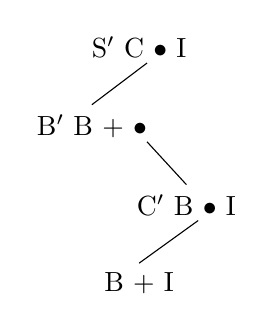
\begin{tikzpicture}
            \node (top)  at (0,0)      {\ml{S$'$ C $\bullet$ I}};
            \node (mid)  at (-0.6,-1)  {\ml{B$'$ B $+$ $\bullet$}};
            \node (low)  at (0.6,-2)   {\ml{C$'$ B $\bullet$ I}};
            \node (bot)  at (0,-3)     {\ml{B $+$ I}};
            \draw (0.1,-0.2) -- (mid.north);
            \draw (0.1,-1.2) -- (low.north);
            \draw (0.75,-2.2) -- (bot.north);
        \end{tikzpicture}%
    }

    \vs
    \hspace{0.5cm}Annotated syntax tree\hspace{2.5cm}Combinator representation
\end{center}

\noindent
The combinator representation is diagrammatic, and when flattened out looks like this:
\begin{mlcoded}
    S$'$ C (B$'$ B $+$ (C$'$ B (B $+$ I) I)) I
\end{mlcoded}
The \ml{I}s in the left-hand tree indicate leaf nodes (they are \textit{bona fide} \ml{I} combinators). Some of these \ml{I}s would not be present in the compiled combinator form because of \te{}-optimization, so if we convert the annotated syntax tree to combinators we would get a slightly suboptimal combinator expression. Notice that not all nodes have the same number of annotations; the bottom node has only one because only \ml{x} gets sent to it.

The simple equivalence between director strings and combinators mentioned above gives a more systematic basis for the choice of combinators we made in the first part of this chapter.

\subsection{Minor Refinements}

Consider the lambda abstraction
\begin{mlcoded}
    \tlb{x}\tlb{y}$+$ y 1
\end{mlcoded}
This does not use \ml{x} at all, so we need a director which says `the argument is not needed in either branch'. We call this director \ml{\underline{j}}. It can only occur at the root of a lambda abstraction, because in the rest of the expression the arguments are only sent where they are needed. Thus the lambda abstraction would have the annotated tree

\begin{center}
    \begin{forest}
        [\phantom{jc }\ml{@ \underline{jc}}
        [\phantom{b }\ml{@ \underline{b}}
        [\ml{$+$}]
        [\ml{I}]
        ]
        [\ml{1}]
        ]
    \end{forest}
\end{center}

\noindent
Corresponding to the director are the \ml{J} and \ml{J$'$} combinators
\begin{letalign}
    J f g x &$\rightarrow$ f g \\
    J$'$ k f g x &$\rightarrow$ k f g
\end{letalign}
Another awkward problem is what to do when given a lambda abstraction such as
\begin{mlcoded}
    \tlb{x}\tlb{y}3
\end{mlcoded}
Here the body is not even an application, so we cannot annotate it. In this case we use the old \ml{K} combinator for the \ml{\tl{}y} abstraction, transforming it to
\begin{mlcoded}
    \tlb{x}K 3
\end{mlcoded}
Now the body is an application, so the annotation for \ml{x} can go as before.

\subsection{Director Strings as Combinators}

We now turn our attention to the implementation of director strings.

So far we have two representations for programs, namely \ml{SK} combinator expressions, and syntax trees annotated with directors. To each director there corresponds exactly one combinator in the combinator representation, each of which takes a whole node. Since there are only four directors (\ml{\underline{j}}, \ml{\underline{s}}, \ml{\underline{b}} and \ml{\underline{c}}), we could encode each director in two bits. Encoding a string of directors as a bit-string would give a dramatic decrease in program size over the combinator representation, since we would need only two bits instead of a whole node to store each combinator. This would make the program execute faster, too, since there would be less of it to fetch from store.

This suggests a third representation of the program:

\begin{center}
    Represent\hspace{0.5cm}%
    \raisebox{-0.5\height}{%
        \begin{forest}
            [\phantom{\underline{vw}\ldots\underline{yz} }\ml{@ \underline{vw}\ldots\underline{yz}}
            [\ml{p}]
            [\ml{q}]
            ]
        \end{forest}%
    }%
    \hspace{0.75cm}as\hspace{0.75cm}%
    \raisebox{-0.7\height}{%
        \begin{forest}
            [\ml{@}
            [\ml{@}
            [\ml{D{vw}\ldots{yz}}]
            [\ml{p}]
            ]
            [\ml{q}]
            ]
        \end{forest}%
    }
\end{center}

\noindent
where \ml{Dvw$\ldots$yz} is one of a family of combinators with the following reduction rules:
\begin{letalign}
    Djvw$\ldots$yz p q x &$\rightarrow$ Dvw$\ldots$yz p q \\
    Dsvw$\ldots$yz p q x &$\rightarrow$ Dvw$\ldots$yz (p x) (q x) \\
    Dbvw$\ldots$yz p q x &$\rightarrow$ Dvw$\ldots$yz p (q x) \\
    Dcvw$\ldots$yz p q x &$\rightarrow$ Dvw$\ldots$yz (p x) q \\
    D &$\rightarrow$ I
\end{letalign}
This new representation, together with the \ml{D} reduction rules, is a perfectly executable combinator program, except that it is represented much more compactly than the original. The only cost is a slight increase in the complexity of the reduction machine. An escape mechanism is also required to deal with the case where there are too many directors in the string to fit in the \ml{D} combinator family. Stoye [1985] describes an implementation of director strings on SKIM.

\section{The Size of {\sffamily SK} Combinator Translations}

One obvious feature of the examples given in this chapter is that the translated program is often much larger than in its lambda form; in fact Kennaway [1982] shows that the size of the combinator expression can be proportional to the square of the size of the lambda expression in the worst case. To become convinced of this, the reader is encouraged to construct the director string form of the lambda abstraction
\begin{mlcoded}
    \tlb{x$_n$}\ldots\tlb{x$_2$}\tlb{x$_1$}(x$_1$ x$_2$ \ldots\ x$_n$)
\end{mlcoded}
A closely related observation is that the \ml{SK} combinator compiler repeatedly re-scans the code it has already partially compiled. This can be seen in the compilation rule
\begin{mlcoded}
    \metafnbb{C}{\tlb{x}e} $=$ \metafn{A} x \doublebracket{\metafnbb{C}{e}}
\end{mlcoded}
in Figure~16.5.

Burton [1982] describes a method for balancing the expression tree, at the expense of introducing extra redexes; this gives a complexity of $O(N\log N)$,
but with a larger constant. Joy \textit{et al.} [1985] summarize these and other related results.

By way of comparison, Hughes [1984] shows that the supercombinator technique has a worst case complexity of $O(N\log N)$, but is typically linear.

To conclude, for a lambda expression of size $N$, \ml{SK} combinator compilation time and code size is worst case $O(N^2)$ and typically $O(N\log N)$, while supercombinator compilation time and code size is worst case $O(N\log N)$ and typically linear.

\section{Comparison with Supercombinators}

\ml{SK} combinators represent one extreme of graph reduction techniques. Complex reductions are reduced to the composition of many fast, simple reductions, so the `grain' of execution steps is about as small as it can conceivably be. This is a mixed blessing, and we attempt a summary of the pros and cons at this point.

\subsection{In Favor of {\sffamily SK} Combinators}

\begin{numbered}
    \item A small, fixed set of combinators can be implemented directly in hardware, thus bypassing a level of interpretation. This is analogous to moving from machine code to microcode.
    \item The instantiation of lambda bodies is done lazily, thus avoiding instantiating sections of graph which are subsequently to be discarded.
    \item The technique is fully lazy.
    \item The reduction machine is relatively simple to implement.
\end{numbered}

\subsection{Against {\sffamily SK} Combinators}

\begin{numbered}
    \item The `grain' of execution steps is too small. Since the arguments to a function are pushed down into its body one level at a time, many intermediate application nodes are created and almost immediately taken apart again. This means that an \ml{SK} combinator reducer consumes a lot of transient storage, which increases the load on the garbage collector.
    \item The translation to combinators is expensive compared with supercombinator techniques, and the resulting program is larger (see Section~16.4).
    \item With \ml{SK} combinators, the larger program increases the number of storage accesses required, as does the creation and subsequent examination of intermediate application nodes.
    \item Any scheme for improving performance using cacheing must operate with a unit of cacheing of a single node. A supercombinator machine can cache whole supercombinator bodies, another consequence of the coarser grain of supercombinators.
\end{numbered}

\section*{References}

\begin{references}

    \item Burton, F.W. 1982. A linear space translation of functional programs to Turner combinators. \textit{Information Processing Letters}. Vol. 14, no. 5, pp. 202--4.

    \item Curry, H.B., and Feys, R. 1958. \textit{Combinatory Logic}, Vol. 1. North-Holland.

    \item Hughes, R.J.M. 1984. The design and implementation of programming languages. PhD thesis, PRG-40. Programming Research Group, Oxford.

    \item Joy, M.S., Rayward-Smith, V.J., and Burton, F.W. 1985. Efficient combinator code. \textit{Computer Languages}. Vol. 10, no. 3/4, pp. 211--24.

    \item Kennaway, J.R. 1982. \textit{The Complexity of a Translation of Lambda Calculus to Combinators}. Department of Computer Science, University of East Anglia.

    \item Kennaway, J.R., and Sleep, M.R. 1982a. \textit{Director Strings as Combinators}. Department of Computer Science, University of East Anglia.

    \item Kennaway, J.R., and Sleep, M.R. 1982b. \textit{Counting Director Strings}. Department of Computer Science, University of East Anglia.

    \item Scheevel, M., 1986. Norma: a graph reduction processor. In \textit{Proceedings of the ACM Conference on Lisp and Functional Programming, Cambridge, Mass.}, pp. 212--19. August.

    \item Stoye, W.R. 1983. The SKIM microprogrammer's guide. \textit{Technical Report 31}. University of Cambridge. October.

    \item Stoye, W.R. 1985. The implementation of functional languages using custom hardware. PhD thesis, Computer Lab., University of Cambridge. May.

    \item Turner, D.A. 1976. \textit{SASL Reference Manual}. University of St Andrews.

    \item Turner, D.A. 1979a. A new implementation technique for applicative languages. \textit{Software -- Practice and Experience}. Vol. 9, pp. 31--49.

    \item Turner, D.A. 1979b. Another algorithm for bracket abstraction. \textit{Journal of Symbolic Logic}. Vol. 44, no. 2, pp. 67--270.

\end{references}